\documentclass[../main.tex]{subfiles}

\begin{document}

\subsection{Solution overview}

The proposed solution consists of two main sections: a drone and a control section. The user will import
the mobility pattern and the constraints to the control section, which is a laptop. Then the user will send high-level commands to the drone agent, which will apply certain operations such as start/stop etc. Once the user finishes importing the mobility pattern and starting the drone mission, the drone will begin to take off and begin to visit the area to scan for getting the most number of mobile targets using \gls{drl} model. Users will keep receiving live updates and the status of service on the control section using Wi-Fi. Most of the connections in the system are wireless, which will have benefits and drawbacks.


\subsection{High level architecture}
Figure 1 shows a high-level architecture of a complete working system, in which a group of connected tools and devices are combined into a single system.In the next section, hardware and software details will be presented in a more detailed way
\begin{figure}[H]
	\centering
	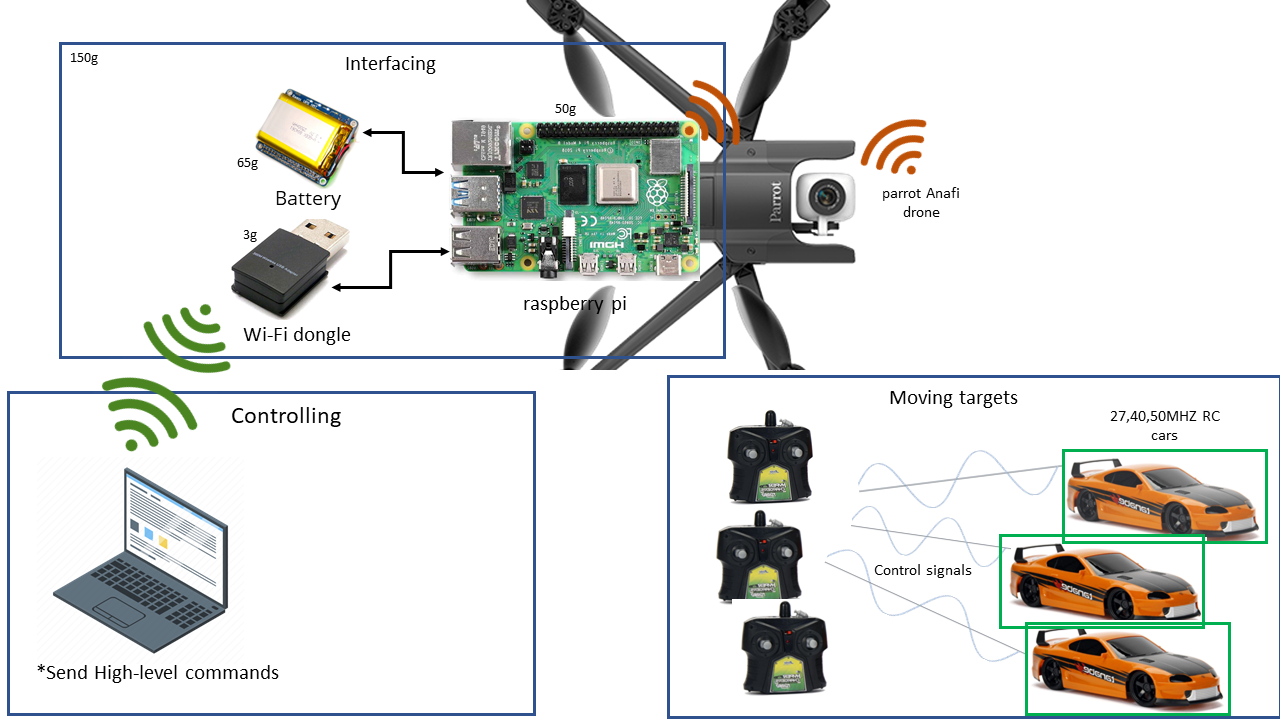
\includegraphics[width=0.9\textwidth]{high-level-arch.png}
	\caption{High-Level Architecture}\label{fig1:arch-fig}
\end{figure}


\subsection{Hardware/software to be used}

\subsubsection{Software}
ubuntu os
parrot olympe
parrot sphinx
Gazebo simulator
roboflow
google colab notebook /jupyter notebook


\subsubsection{Hardware}
Parrot ANAFI Drone
Raspberry Pi 4
lithium Battery
Wi-Fi adapter dongle
laptop control station

\end{document}
